\documentclass[a4paper,12pt]{article}
\usepackage{amsmath}
\usepackage{amssymb}
\usepackage[utf8]{inputenc}
\usepackage[T1]{fontenc}
\usepackage{lmodern}
\usepackage{indentfirst}
\usepackage{geometry}
\usepackage{array}
\usepackage[pdftex]{color,graphicx}
\usepackage{subfigure}
\usepackage{afterpage}
\usepackage{setspace}
\usepackage{color}
\usepackage{wrapfig}
\usepackage{listings} 
\usepackage{datetime}
\usepackage{epstopdf}
\usepackage{hyperref}

\renewcommand{\onehalfspacing}{\setstretch{1.6}}

\geometry{tmargin=2.5cm,bmargin=2.5cm,lmargin=2.5cm,rmargin=2.5cm}
\setlength{\parindent}{1cm}
\setlength{\parskip}{0mm}

\newenvironment{lista}{
\begin{itemize}
  \setlength{\itemsep}{1pt}
  \setlength{\parskip}{0pt}
  \setlength{\parsep}{0pt}
}{\end{itemize}}

\newcommand{\linia}{\rule{\linewidth}{0.4mm}}

\definecolor{lbcolor}{rgb}{0.95,0.95,0.95}
\lstset{
  backgroundcolor=\color{lbcolor},
  tabsize=4,
  language=C++,
  captionpos=b,
  tabsize=3,
  frame=lines,
  numbers=left,
  numberstyle=\tiny,
  numbersep=5pt,
  breaklines=true,
  showstringspaces=false,
  basicstyle=\footnotesize,
  identifierstyle=\color{magenta},
  keywordstyle=\color[rgb]{0,0,1},
  commentstyle=\color{green},
  stringstyle=\color{red}
  }

\begin{document}

\noindent
\begin{tabular}{|c|p{11cm}|c|} \hline 
Michał Szczygieł & Aleksander Śmierciak & \ddmmyyyydate\today \tabularnewline
\hline 
\end{tabular}


\section*{Zadanie 3 - Trigramy - Analiza dokumentów}

Programem spełniającym polecenie zadania 3. jest taki, który przyjmując listę plików wejściowych, przeanalizuje ich zawartość tworząc mapę dystrybucji n-gramów o rozmiarze 3 (trigramów).
\\

Część kodu odpowiedzialna za uzupełnienie informacji o częstości występowania trigramów w tekście źródłowym prezentuje się następująco:

\begin{lstlisting}
    #pragma omp parallel
    {
        unsigned int threadNumber = omp_get_thread_num();
        unsigned int startPos = chunkSize * threadNumber;
        unsigned int endPos = chunkSize * (threadNumber + 1);
        endPos = std::min(endPos, (unsigned int)contents.size());
        for (unsigned int i = startPos; i < endPos; i += 3)
        {
            string trigram = contents.substr(i, 3);
            ++trigramDistribution[trigram];
        }
    }
\end{lstlisting}

Wcześniejsza implementacja:

\begin{lstlisting}
	#pragma omp parallel num_threads(threadCount)
	{
		std::string threeLetters;
		unsigned int endPosition = portion * (omp_get_thread_num() + 1);

		if (endPosition > contents.size())
		{
			endPosition = contents.size();
		}

		#pragma for default(none) shared(contents, trigram) firstprivate(portion) private(threeLetters)
		for (int i = portion * omp_get_thread_num();
				i != portion * (omp_get_thread_num() + 1); i += 3)
		{
			threeLetters = std::string(contents.substr(i, 3));
			trigram[threeLetters]++;
		}
	}
\end{lstlisting}

Była podatna na błędy współbieżnego dostępu do mapy wystąpień trigramów, a także jej wydajność była dużo niższa. Wynikało to zapewne z tego w jaki sposób dane są porcjowane – porcjowanie ręczne pozwala na większą kontrolę nad rozmiarem porcji, co więcej, pozwala ustawić nieregularny rozmiar porcji, co jest szczególnie przydatne, gdy rozmiar danych wejściowych nie jest podzielny przez 3 * [liczba wątków].
\\

Niestety kolekcje standardowej biblioteki szablonów nie są przystosowane do pracy w architekturze wielowątkowej; ich metody nie są pod tym względem bezpieczne. Aby móc bezpiecznie stosować te metody należy zaimplementować własne mechanizm kontroli dostępów (np. zamki), albo zastosować sekcję krytyczną (\emph{pragma omp critical}).


\section*{Przebieg}
Obliczenia zostały wykonane na serwerze CUDA. \\



Poniżej wykresy przedstawiający rezultat przeprowadzonych operacji na wątkach.
\\
\begin{center}
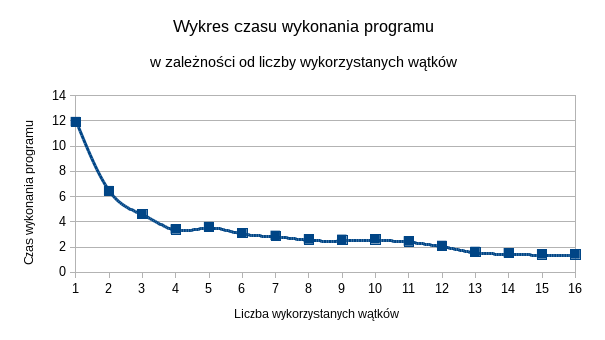
\includegraphics[width=0.7\textwidth]{data/wykonanie.png}
\end{center}


\begin{center}
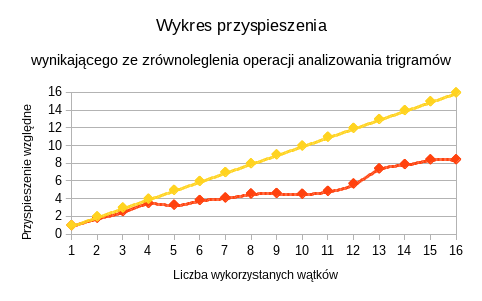
\includegraphics[width=0.7\textwidth]{data/przyspieszenie.png}
\end{center}

Wykresy z zaimplementowanymi zamkami.
\\
\begin{center}
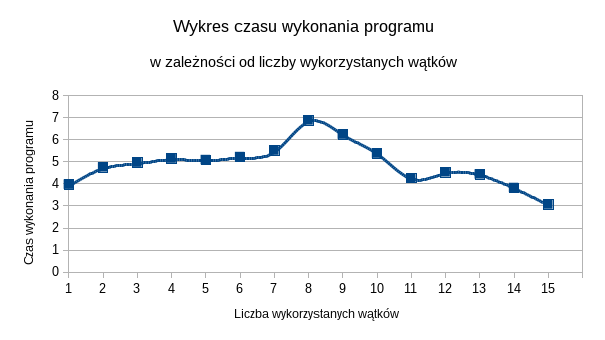
\includegraphics[width=0.7\textwidth]{data/wykonanie_2.png}
\end{center}


\begin{center}
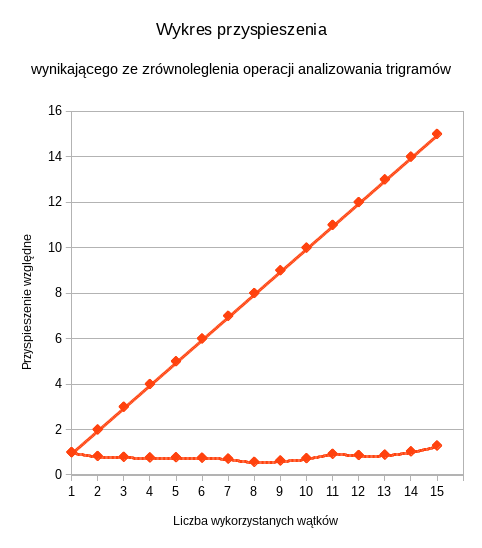
\includegraphics[width=0.7\textwidth]{data/przyspieszenie_2.png}
\end{center}

\section*{Wnioski}
Zauważalny spadek wydajności można tłumaczyć liczbą rdzeni maszyny, na której wykonywano pomiary (serwer CUDA) oraz sposobem przydziału zadań – algorytmem karuzeli – klauzula schedule(static).

\end{document}